%!TEX root = main.tex

\section{StarCraft}
\label{sec:starcrafttheory}
\begin{figure}[h!tb]
\centering
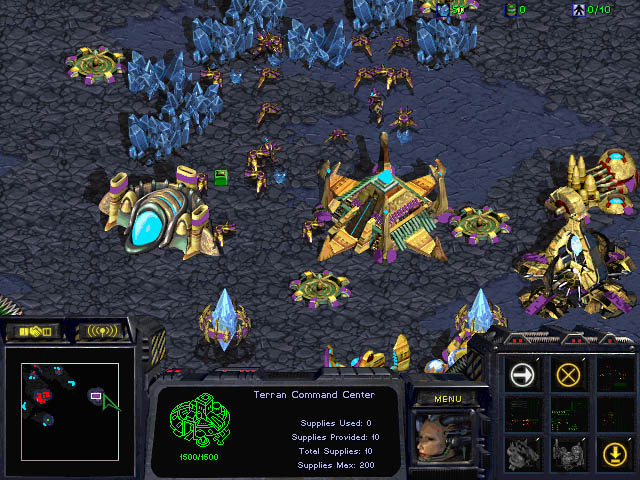
\includegraphics[scale=0.5]{graphics/scbw.jpg}
\caption{StarCraft: Brood War}
\label{fig:scbwIntro}
\end{figure}

StarCraft is a military science fiction real-time strategy developed by Blizzard
Entertainment in 1998.\cite{starcraft} The game has a single-player campaign,
but it is most famous for its one vs. one multi-player where the goal is to
defeat an opponent on the battlefield, using one of three distinctive races;
the earth-originated Terrans, the advanced Protoss or the hive-minded,
insectoid Zerg. StarCraft: Brood War is an expansion pack for the original
StarCraft that introduces new units, upgrades and maps. 

A typical multi-player game starts with each player choosing their race and the
selection of a map to fight on. Each player are then spawned in one of
several potential start locations. If the map has more than two start
locations, they don't know where the enemy spawns and will have to go look for
them. Each player is given a foundation building and a few workers at the
beginning of the match, and how the rest of the match then unfolds are now up
them. A match consists of gathering resources and securing one or more bases in
order to produce units for an army that can be used to defeat the enemy. Victory
in the match is achieved by killing all of the opponents structures or forcing
them to concede.

The resources in the game are minerals and gas. Minerals are mined from mineral
formations that are found in each base location, and placing the foundation
building close to them is important so the workers do not have to move to far
when they collect minerals. Gas is extracted from geysers that are found next to
the mineral formations, but in order to harvest it a player must build a
specific structure on top of the geyser. Afterwards, workers can collect gas in
the same way they collect minerals. Each base location has a limited amount of
minerals, and in order to continue to acquire minerals a player must expand to
another base by building a new foundation building at that location. Taking
several bases at the same time allows for increased income and greater unit
production. But there are a limited amount of minerals on the map which will
force a match to end in a reasonable amount of time (towards the end players
won't be able to resupply their armies). Gas on the other hand never runs out,
but after a certain threshold of gas collected from it, gas will be collected at
a reduced rate of 1/4 of the original one.

StarCraft is on the surface a very simple game, it has only three different
playable races, a handful of different buildings and units, and with goals that
are relatively simple to comprehend. But once you start analyzing the game, the
reality is quite different. The Brood War expansion pack was released back in
1998, and the game has been played at a competitive, high level since then and
all the way up to today. And the metagame\footnote{Metagame is a description of
the part of the game that transcends a single match, for example popular
strategies, tactics, counters to these, at a given time.} has evolved during the
entire lifespan of the game and is still changing today with new tactics showing
up from tournament to tournament. \cite{starcraft}

When playing at a high level you are working with really small windows of
opportunity, often called timings. And it is these timings that enable a game
with what should in theory be simple elements to have such complex and evolving
strategies. The effectiveness of an attack on the enemy bases can be decided by
the presence of a single important unit, so if this unit is produced 20 seconds
to late the attack could have crushed the defending army and started killing
buildings by the time that unit is finished. When playing with so small margins
every little change can have massive consequences on the outcome of the match,
and this creates the high level of dynamic play that StarCraft is known for.
 
\subsection{Macro and Micro}
Macro-management and micro-management, henceforth referred to as \textit{macro}
and \textit{micro} respectively, are the two concepts that you have to master
in order to play StarCraft, or any other RTS, at a successful level. These
concepts incorporate everything from low level control of units to the high
level strategy and tactics used in a game. And finding a good balance between
them are one of the main challenges about playing RTS games for human players.
Micro is the ability to control individual or group of units in an efficient
way. Having better micro than your opponent enables you to win fights where you
have an equal or even outnumbered army. Good micro enables you to 
compensate for poor in-game AI/path finding by individual control of the
units, this also allows you to save more units that are taking heavy fire and to
focus down important targets in the enemy army. Macro is the ability to produce
units and construct new buildings at the appropriate times. Good macro means you
are always producing something with your buildings and and that you expand or
increase your production capacity at appropriate times when you have the
resources to support this. The player that has the best macro usually have the
biggest army when the time to battle comes. While it is best to have both great
macro and great micro, this is usually not possible, so players have to choose
where they spend to use their attention. Because good macro means you will have
a better economy and more units it is generally agreed that macro is more
important then micro, though it is important to have a good balance of both in
order to play at a high level.

\subsection{Supply}
In StarCraft there is always a limit to how many units a player can have at a
given time. This is called supply for terran, control for zerg and psi for
protoss. They function the same way for every race, so most people just call it
supply no matter what race they are talking about. Each race has a building or
unit that can increases their possible supply count up to a maximum of 200.
Terran has a building called the supply depot, protoss has a building called a
pylon and zerg uses a flying unit called an observer. More powerful units have a
larger supply demand then basic units, so you you can have less of them before
you run out of available supply. It is therefore important to find a balance
between basic and advanced units that gives you an good sized army but also with
powerful units. Because zerg have more basic units, and protoss have more
advanced units it is very normal for a zerg player to have a greater army size
and the protoss to have a smaller army but with more powerful single units.
 
Supply blocked is what happens when a player can't create any more units because
he has reached his maximum supply. This can happen when a player forgets to
build more supply buildings/units as he is creating new units, or an enemy
destroys one or more of the buildings/units that increases the supply count.
Being supply-blocked can have big consequence as it gives the other player an
edge to exploit because you can't create any more units until the supply is
increased by creating new supply buildings/units. This small edge can be just
what the enemy needs to pull ahead in the game and get a victory. Because of
this players will often launch hit and run attacks that are aimed at supply
blocking the opponent.
 
\subsection{Fog of War and Scouting}
StarCraft is a game with imperfect information, meaning you do not see
everything that is happening on the map. The map is covered by a \textit{fog
of war} that hides what is happening. Any unit or structure that you own reveals
an area around itself where you can see everything. Because of this scouting
becomes a very important aspect of playing StarCraft. Scouting means sending a
unit out to places on the map where you don't know what is happening, the most
important area being the opponents base, but also to make sure he has not placed
buildings or hidden armies someone else on the map. Early game it is very common
to send a worker unit out to look around the opponents base in order to gather
information on what he is doing and what strategies he is working towards so
that you can counter this. This also means that denying the opponent scouting
information at critical stages in the game is an important aspect, for instance
hiding that you are building air units so that you can launch a surprise attack
that will catch them unprepared. Other ways to exploit the fog of war is to
create hidden expansions\footnote{Extra foundation buildings used to generate
additional income from other mineral patches or gas geysers.}, or hide important
buildings so it is more difficult for your enemy to figure out what strategy you
are going to use. 

\subsection{Races}

\subsubsection{Terran}

Terran are the human faction of StarCraft, a futuristic version of man today.
They are known for high adaptability with a good variety of defensive and mobile
armies. They are best known for their mobile biological armies, or their slow
moving turtling tech(tanks) armies that slowly creeps across the map and secures
section by section. This versatility makes them a great class with a lot of
different possible strategies and combinations that can be effective.
 
The Terran worker is the Space Construction Vehicle (SCV). This unit can gather
minerals, build buildings and, unique for the Terran race, repair other
mechanical units or buildings. When constructing buildings the unit has to work
on the building from the initial placement to the building is complete, meaning
it will be unable to perform other action in this time, and can be attacked. If
the SCV halts construction or is killed, the building will have to be canceled
or finished by another SVC. Like mentioned before it can also repair mechanical
units like tanks if they have taken damage, but to perform this action they have
to be pulled from other tasks like mining minerals so it is a two edged sword.
Terran buildings will slowly self destruct if left at low health, so it is
important to repair them if they have taken significant damage.
 
Terran buildings also have a unique feature in that they can lift of the ground
and fly around after being constructed. They can then land in a new location and
continue production of units or upgrades. Some buildings can also create add-ons
that unlocks new units and upgrades for that building. Terran also have a unique
building in the bunker. This a defensive building where  biological units can
seek refuge while still attacking, but from a fortified position that protects
them from damage. The bunker has to be taken out before the units inside can be
damaged and killed. While being useless on it's own, the building can be a death
trap when filled with infantry. The bunker can also be repaired by an SCV, like
any other Terran building, so the SCVs have to be a priority for an attacking
army before they can destroy the bunker.
 
The health regeneration mechanics for the Terran race are twofold. The medic is
used to heal biological units after they have suffered damage in battle (they
can also heal other medics, but not themselves). Mechanical units can be
repaired by pulling SCVs, for example from mining, and using them to repair the
unit. SCVs can also be effective to use in combat as they can repair the unit
while it is taking damage, and several SCVs can repair the same unit at the same
time for an increased regeneration rate.
 
\subsubsection{Protoss}
The protoss are a technologically advanced alien race that rely on psionic
abilities and cybernetics in battle. Because they are the most technological
advanced race in StarCraft they are known for their raw power. With powerful but
expensive units they can crush their opponents on the battlefield even if they
are outnumbered army because of superior firepower.

The protoss worker is called a probe, and is like the SCV used to gather
minerals and build buildings. Protoss buildings are not constructed, but warped
in from their home planet, so a probe only needs to place a warp beacon where
the building should be placed and then it can return to mining minerals while
the building warps in by itself. This allows the use of one probe for
construction of several buildings at basically the same time, and then it can
return right to mining. This can allow an protoss player to setup remote
expansions in a short time with a single probe. 

In contrast to the terran race the protoss can't just build buildings anywhere,
they have to place them on a power grid generated by a pylon, the protoss supply
building. Pylons also power buildings, so if an enemy takes out all the pylons
around some production building it can no longer produce any units or research
upgrades. The player will then have to build new pylons to power up the building
again before he can continue production. 

Special for protoss units and buildings are that they have energy shields that
protect them against damage and recharges to full strength over time. In order
for an enemy to damage a protoss unit, it has to first deplete the shield that
protects it, only then can they proceed to damaging the unit itself. For an
enemy it is therefore important to finish of the unit when it's shield is fully
depleted or it will regenerate to full strength. 

\subsubsection{Zerg}
The zerg are not actually a race of its own, but rather a collection of very
different creatures and races that have been assimilated and united under a
central intelligence called the Overmind. Striving for power, they have been
selectively evolved towards being very effective killers. Technologically they
are far behind the other races, but they make up for this with a big army size
and superior biological properties. 

The zerg worker unit is called a drone. When constructing a building a drone
will ``sacrifice'' itself and mutate into the building. This means that for
every building that the player constructs he loses a worker. In every other way
they behave just the same as the worker units for the other races. For every
race the worker unit is produced from the foundation building, for zerg this is
the hatchery. But for zerg every other unit is also created from the hatchery,
and any unit buildings that are constructed only unlocks the possibility to
create that unit from the hatchery. This is because zerg have a special game
mechanic called larva. These special non-controllable units are produced by the
hatchery over time, up to a maximum of three at a given time, and they can be
morphed into another zerg unit that is unlocked (units they can be morphed into
depends on what buildings the zerg player has built).

Similar to protoss the zerg can't just build buildings anywhere, because the
buildings are biological they require nourishment to function, and have to be
built on creep. Creep is produced by the Hatchery and Creep Colonies and then
radiates outwards from these onto any fertile ground in the area. The Hatchery
is the only building that can be built without creep, as it produces its own
nourishment. 

Zerg units and buildings have a unique ability to regenerate lost health over
time if left alone. This means an attacker should finish off an attacked unit or
it will come back with full health after a while. This also makes tactical
retreats much more important for the zerg players, as they can then rest their
army to allow them to regenerate back to full health after taking damage in a
battle. Burrowing is also a unique ability for the zerg units, and has great
synergy with the health regeneration ability. This allows them to burrow in the
ground to get out of harms way, and here they can regenerate health without
worrying about taking damage. This also allows for ambush tactics by burrowing
armies and waiting for the enemy before launching a surprise attack. It can even
be used to gain map control by burrowing units in strategic places to scout that
area. Only using some form of detector can the enemy see and attack units that
have burrowed. 

\subsection{BWAPI}
The Brood War Application Programming Interface (BWAPI)\cite{bwapi} is an open
source C++ framework project for creating AI modules for StarCraft: Brood War.
BWAPI is a third party ``hack'' of StarCraft: Brood War to allow programmers to
retrieve and send information to the game at real-time. The API provides the
programmer with information about the game state and the individual units, as
well as allows them execute actions similar to what a normal player would be
able to perform. 

There are a two different ways to ``inject'' an agent into StarCraft; it can be
made as a module that gets loaded into StarCraft or as a standalone process that
communicates with BWAPI through a shared memory area, a client-server approach.
What method to use depends on several factors, but mainly what language that
will be used. Because BWAPI (and StarCraft itself) is written in C++ the module
that gets ``injected'' have to be in the same language, but the client-server
approach much more easily enables other languages to be used as the client side
is independent and can be written in any language that has a port of the BWAPI
protocol. This includes several languages such as Java, C\#, Python and F\#.
The API also supports several degrees of accessibility, meaning you can play a
game as a normal real player would with limited information, or you can start a
game that is fully observable. The later is mainly of academic interest, where
you want to test an AI that requires a fully observable environment.

The API provides extensive and detailed information about the game state,
basically anything a player can see in a game is also available though the API.
Some examples of this are unit locations, production times, available
structures, cost of buildings and units. In some cases the API even provides
additional information that is not available to a human player in the game, this
can be the exact unit speed and the damage and armor of a unit. This is
information that a player usually learns outside the game, but for an AI agent
it makes it easier for the developer, as a lot of domain knowledge can be
retrieved from the API as apposed to having to bundle this in every agent. 

\subsubsection{BWSAL}
BWAPI Standard Add-on Library (BWSAL)\cite{bwsal} is a project that have created
several add-on to the standard BWAPI. The project aims to be a foundation for
creating AI agents with BWAPI. The main parts of the Library are managers that
handles a lot of the boiler plate code that is required to get a functional
agent with BWAPI. Features like finding available locations where one can
construct a building, basic control of units and workers, scouting and build
order managers are available. A lot of this code would be quite similar and time
consuming to create for each AI agent, so using the add-on library one can much
easier get a working agent up and running and the developers can start focusing
on their main priorities. 

\subsubsection{BWTA}
The Brood War Terrain Analyzer (BWTA)\cite{bwta} is another add-on for BWAPI
that is used for analyzing the terrain in StarCraft maps. BWTA calculates
regions, choke points and base locations on the given map. The calculations are
done before the match, and the results can then be accessed and used by the
agent as it sees fit.  